\chapter{Sprint 8 - Summary}

In sprint 8, the team has started to flight test and tune the PID-values of the quadcopter. To reduce the chances of damage to the vehicle, all flight testing has been performed on pillows. 
\\
Vibrations are still a challenge, small mechanical variations gives a huge impact on the noise registered by the IMU. To reduce noise, mechanical fine tuning of the mechanisms, motor alignment and filtering in software has been done. 
\\
The servos makes a cyclic twitchy sound. The issue has been investigated thoroughly, but no apparent reason has been identified. The conclusion is that it is caused by hardware limitations in the Arduino Nano.
\\
In the flight controller, the start RPM of the motors have been increased. This is done to achieve a more agile flight regime. Operating on higher RPMs will ensure that as much kinetic energy as possible is stored in the propellers for when pitch is actuated. The RPM max value is limited to 50-60\%, values above this have shown to give excessive vibrations and hence noise.
\\
In this sprint, documentation has been in focus. Old documents are reviewed and proofread, and other documents are being completed. The main thesis document has been started and will be merged as documents finished.
\\
The quadcopter has been test flown by a professional RC-pilot. According to him, the feel of the quadcopter was more responsive than what he had experienced with regular fixed pitch.

\section{Completion and Scope Change}

In sprint 8, 100 \% of all planned tasks were completed and there was no changes in scope

\begin{figure}[H]
    \centering
         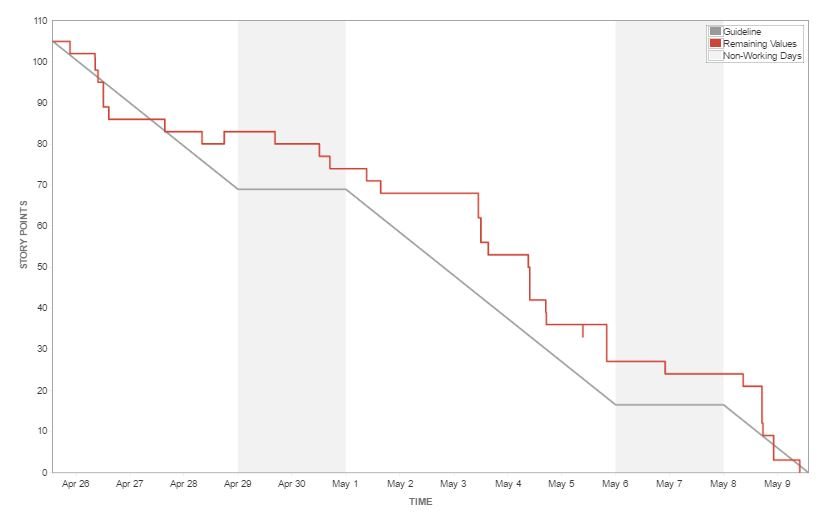
\includegraphics[width = 1\textwidth]{VAPIQ-PICTURES/BDSprint8}
      \caption{Burndown Chart Sprint 8}
    \label{fig:bds8}
\end{figure} 

\textbf{Project plan status, Sprint 8:}
\begin{itemize}
        \item Final Flight Controller Adjustment , \textbf{In progress}
        \item Mechanical Improvements, \textbf{In Progress}
        \item Documentation , \textbf{In progress}
        \item Testing And Comparison, \textbf{Postponed}
    \end{itemize}

% Vibrations-> Filters-> Mechanical Noise Reduction, etc
% Servo twitch, probably timer issues--> not resolved--> tried with mega with additional timer--> did not work
% Modeld Pitch-> High Start RPM, small compensations in RPM when chaging the pitch. Maximize kenetic energy
%PID-tuning!!!!!!!!!!!!!!!!!!!!!!!!!!!!!!!!!!!!!!!!!!!!!!!!!
%Flight testing!!!!!!!!!!!!!!!!!!!!!!!!!!!!!!
%Documentation%%%%%%%%%%%%%%%%%%%%%%%%%
%

